\documentclass{resume}

\usepackage{dejavu}

\usepackage{hyperref}
\hypersetup{
	colorlinks=true,      
	urlcolor=blue,
}

\urlstyle{same}

\begin{document}

\noindent
\begin{tabularx}{\linewidth}{@{}m{0.82\textwidth} m{0.18\textwidth}@{}}
{
    \large{Смородинов Александр Андреевич} \newline
    \small{
        \clink{
            \href{mailto:asmorodinov66@gmail.com}{asmorodinov66@gmail.com} \textbf{·} 
            \href{https://github.com/asmorodinov}{github.com/asmorodinov} \textbf{·} 
            \href{https://t.me/asmorodinov}{tg: @asmorodinov}
        } \newline
        Москва, Россия
    }
} & 
{
    \hfill
    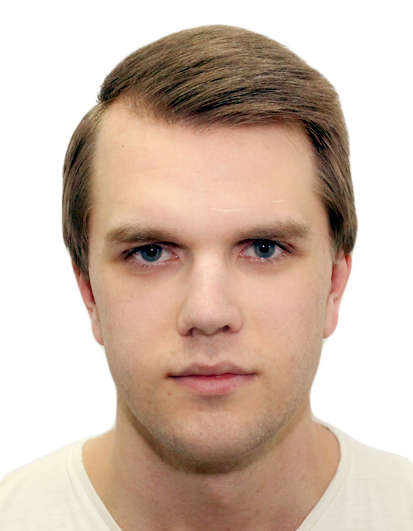
\includegraphics[width=2.95cm]{images/photo.jpg}
}
\end{tabularx}

\begin{center}
\begin{tabularx}{\linewidth}{@{}*{2}{X}@{}}
% left side %
{
    \csection{Опыт работы}{\small
        \begin{itemize}
            % item 1 %
            \item Стажировка в \href{https://luden.io/}{luden.io}, лето 2021
            \item Работа над игрой \href{https://luden.io/craftomation/}{Craftomation 101} в \href{https://luden.io/}{luden.io}, зима 2021-2022
            \item Стажировка в \href{https://luden.io/}{luden.io}, лето 2022
        \end{itemize}
    }
    \csection{Образование}{\small
        \begin{itemize}
            % item 1 %
            \item \frcontent{Студент 4 курса ФКН} {Прикладная Математика и Информатика}{Распределенные системы}{НИУ ВШЭ}{2019-2023}
            \item \frcontent{Курсы по языкам Rust и Golang}{}{}{ШАД}{2021-2022}
            \item Окончил ГБОУ \small{Лицей ''Вторая школа''} \newline 2019
        \end{itemize}
    }
    \csection{Достижения}{\small
        \begin{itemize}
            % item 1 %
            \item \frcontent{Всероссийская олимпиада школьников по математике}{участник заключительного этапа}{}{2019}
            % item 2 %
            \item \frcontent{Турнир Городов (международная математическая олимпиада)}{}{3 диплом}{2019}
            % item 3 %
            \item \frcontent{Московская математическая олимпиада школьников}{2 диплом}{}{2019}
        \end{itemize}
    }
	\csection{Хобби и интересы}{\small
		\begin{itemize}
			\item 3D графика
			\item Программирование игр
		\end{itemize}
	}
} 
% end left side %
& 
% right side %
{
    \csection{Навыки}{\small
        \begin{itemize}
            \item \textbf{Языки программирования} \newline
            {\footnotesize C/C++, GNU assembler x86, Rust, Golang, Python, Lua, Javascript, SQL}
            \item \textbf{Технологии} \newline
            {\footnotesize Docker, TCP, UDP, gRPC, RabbitMQ, AMQP, Redis, REST API, GraphQL}
            \item \textbf{C++ Библиотеки} \newline
            {\footnotesize GLFW, GLAD, Dear ImGui, Assimp, SFML, Bullet Physics, EnTT}
            
        \end{itemize}
    }
    \csection{Проекты}{
        \begin{itemize}
            \item \small 3D рендерер \newline \footnotesize \clink{\href{https://github.com/asmorodinov/3d-renderer-from-scratch}{github.com/asmorodinov/3d-renderer-from-scratch}}
           	Проект был написан в рамках курсовых работ 2 и 3 курса.
            На 2 курсе был реализован программный 3D рендерер с нуля, с минимальным количеством сторонних библиотек, а на 3 курсе была добавлена поддержка более продвинутых алгоритмов отрисовки. \newline C++
            
            \item \small Сетевая игра мафия \newline \footnotesize \clink{\href{https://github.com/asmorodinov/mafia_graphql_service}{github.com/asmorodinov/mafia\_graphql\_service}}
            Проект был реализован в качестве домашних заданий по курсу ''Сервис-ориентированные архитектуры'' (3 курс ФКН).
           	В игре есть голосовой чат, регистрация пользователей через REST сервис. Пользователи могут редактировать свои профили и получать статистику по играм в формате PDF. GraphQL сервис позволяет просматривать список игр и добавлять комментарии к играм.  \newline Python, Go
            
            \item \small Клон игры Астероиды \newline \footnotesize \clink{\href{https://asmorodinov.github.io}{asmorodinov.github.io}} \newline
            \footnotesize \clink{\href{https://github.com/asmorodinov/asmorodinov.github.io}{github.com/asmorodinov/asmorodinov.github.io}}
            Школьный проект, был написан на уроках информатики в 11 классе за пару недель. \newline
            Javascript
        \end{itemize}
    }
}

\end{tabularx}
\end{center}
\end{document}
